\documentclass[protokoll]{dvd}
\usepackage{graphicx}
\usepackage{pdfpages}
\KOMAoptions{
	headwidth = 18cm,
	footwidth = 18cm,
}

\setlength{\parskip}{0.2em}

% Styrelsen
\def\ordf{Daniell Cole}
\def\vice{\vak}
\def\samo{\vak}
\def\kassa{Owais Tabbaa}
\def\sekr{\vak}

\def\vak{\emph{vakant}}

% mötesinfo

\def\nr{1}
\def\yr{2026}
\def\ymd{2026-04-01}
\def\starttime{17:29}
\def\loc{EA}

% formalia
\def\kall{2026-03-18}


\begin{document}

\title{Divisionsstämmans möte \nr}
\subtitle{\yr}
\author{Divisionsstämman}
\date{\ymd}

\textbf{Datum:} \csname @date\endcsname\\
\textbf{Tid:} \starttime\\
\textbf{Plats:} \loc\\
\textbf{Styrelsemedlemmar:}
\begin{närvarande_förtroendevalda}
    \förtroendevald{Ordförande}{\ordf}{Ja}
    \förtroendevald{Vice ordförande}{\vice}{---}
    \förtroendevald{SAMO}{\samo}{---}
    \förtroendevald{Kassör}{\kassa}{Ja}
    \förtroendevald{Sekreterare}{\sekr}{---}
\end{närvarande_förtroendevalda}

\textbf{Närvarande övriga medlemmar:}
\begin{närvarande_medlemmar}
    \medlem{Sarah Manktelow}
    \medlem{Alexander Appelin}
    \medlem{Ola Forss}
    \medlem{Halimo Hassan Ali}
    \medlem{Edvin Lundgren}
    \medlem{Tural Binnatov}
\end{närvarande_medlemmar}
\newpage

\section{Öppnande av möte}
Mötet beräknas öppnas av \ordf \ \starttime


\newpage
\section{Formalia}

\subsection{Fastställande av röstlängd}
En röstlängd är en lista på personer som har rösträtt. Under våra stämmomöten äger endast divisionsmedlemmar som närvarar vid mötet rösträtt. Därmed krävs det att för att stämmomötet ska kunna genomföras behöver vi en lista med namn på röstberättigade medlemmar som närvarar vid stämmosammanträdet.

Medlemmar kan under mötets gång, det vill säga efter denna punkt, läggas till eller tas bort ur röstlängden.
Det ska då framgå i röstlängden vid vilken punkt i mötesschemat medlemmen lämnar eller ankommer till
stämmomötet.

\subsubsection*{Förslag till beslut}
\begin{attsatser}
    \item stämman fastställer den nuvarande röstlängden
\end{attsatser}

\subsubsection*{Beslut}
\begin{attsatser}
    \item attsats 1 bifalles.
\end{attsatser}


\subsection{Divisionsstämmans beslutbarhet}

6 kap. i stadgan definierar regler Divisionstämman.

\kall \ 
kallade styrelsen till divisionsstämma genom att skriva i discordservern \emph{MonadenDV}, samt annonserades detta på \emph{dvet}.se \kall

\subsubsection*{Förslag till beslut}

\begin{attsatser}
    \item divisionsstämman har uppnått kraven i stadgan för att få hålla möte, och är därmed beslutbar.
\end{attsatser}

\subsubsection*{Beslut}
\begin{attsatser}
    \item attsats 1 bifalles.
\end{attsatser}


\subsection{Fastställande av mötesschema}

För att divisionsstämman ska kunna fatta ett beslut eller protokollföra en diskussion behöver punkten i mötesschemat där stämman ska fatta beslut vara inlagd eller föras in i mötesschemat senast vid den här punkten.

\subsubsection*{Förslag till beslut}

\begin{attsatser}
    \item mötesschemat fastställs utan några ändringar.
    %\item lägga till \textit{punkt vid sektion ...}
\end{attsatser}

\subsubsection*{Beslut}
\begin{attsatser}
    \item attsats 1 bifalles.
\end{attsatser}

\subsection{Val av mötesordförande}

Mötesordförande har till uppgift att leda Divisionsstämmans sammankomst.
Hen ansvarar för att mötesformalia sköts.


\subsubsection*{Förslag till beslut}
\begin{attsatser}
    \item \ordf\ väljs till mötesordförande.
\end{attsatser}

\subsubsection*{Beslut}
\begin{attsatser}
    \item attsats 1 bifalles.
\end{attsatser}

\subsection{Val av vice mötesordförande}

Vice mötesordförande hjälper mötesordförande med att hålla talarlistan, och att alla får komma till tals.

\subsubsection*{Förslag till beslut}
\begin{attsatser}
    \item \kassa\ väljs till vice mötesordförande
\end{attsatser}

\subsubsection*{Beslut}
\begin{attsatser}
    \item attsats 1 bifalles.
\end{attsatser}

\subsection{Val av mötessekreterare}

Mötessekreteraren har till uppgift att anteckna diskussioner, beslut, och eventuella reservationer under mötet.

\subsubsection*{Förslag till beslut}
\begin{attsatser}
    \item \ordf\ väljs till mötessekreterare
\end{attsatser}

\subsubsection*{Beslut}
\begin{attsatser}
    \item attsats 1 bifalles.
\end{attsatser}

\subsection{Val av protokolljusterare}

Protokolljusterare har till uppgift att kontrollera att protokollet i slutändan reflekterar de faktiska besluten och diskussionerna som fördes under sammanträdet; samt agera rösträknare vid slutna omröstningar.
Utöver protokolljusterarna så ska mötesordförande och mötessekreteraren signera protokollet.
Vid Divisionsstämmans sammanträden ska det vara två justerare.\\
Mötesordförande och mötessekreteraren kan inte vara justerare.

\subsubsection*{Förslag till beslut}
\begin{attsatser}
    \item Sarah Manktelow väljs till protokolljusterare
    \item Alexander Appelin väljs till protokolljusterare
\end{attsatser}

\subsubsection*{Beslut}
\begin{attsatser}
    \item attsats 1 \& 2 bifalles.
\end{attsatser}

\newpage

\section{Rapporter}

\subsection{Styrelsen}

\subsubsection*{Ordförande}
Det har varit lite kaosartat och stressigt men jag har överlevt och kandidatarbetet rullar på.\\
Jag har deltagit på diverse möten med göta, bland annat så ska studentrepresentation nu vara tillbaka på banan. Tydligen hade Petrus inte sparat någon info om studentrepresentanter eller om vilka som var kontaktpersoner på institutionen och programansvariga. 

Knapptryckarkompaniet fick 23 röster, vilket ledde till 1 (en) plats i FUM och därmed är jag fullmäktigeledamot i Göta studentkårs fullmäktige för verksamhetsåret 2026/27! 
Perioden att rösta var under vår tentavecka och jag glömde då skicka ut meddelanden om detta för jag var stressad med plugg. 

Har deltagit på så många möten med göta som jag kunnat, där jag försökt bygga broar och bygga positiva intryck med de andra NaTsek föreningarna. Under möten med tema inspark har jag också tryckt på att ha fler programmdagar. 

Snart dags att förnya föreningsstatus så förvänta er en ett utskick om medlemskap snarast. 

 - Daniell Cole, Ordförande '26

\subsubsection*{Kassör}
Nu var det inte så mycket som hänt eftersom har jag ingen tillgång till dv bankkontot än dock efter 10+ meddelande fram och tillbaks med matti och med hjälp av hannes hade vi äntligen köpt ett steam deck för monaden, men (förhoppningsvis) snart ska jag kunna göra mer kassöraktig arbete efter jag tar över kassan.

\subsection{Verksamhetsrapporter: Kommittéer}

\subsection{Studienämnden}
Vi har inte haft officiella studentrepresentanter hela läsåret (I blame Petrus) men förhoppningsvis ska det bli bättre med det i framtiden.

Planerar också mittkurs-utverderingsfika-kombo-pluggstuga????
\\
\ \ - Daniell "Cassilda"
% Alex ställer upp

\subsubsection*{DVRK}
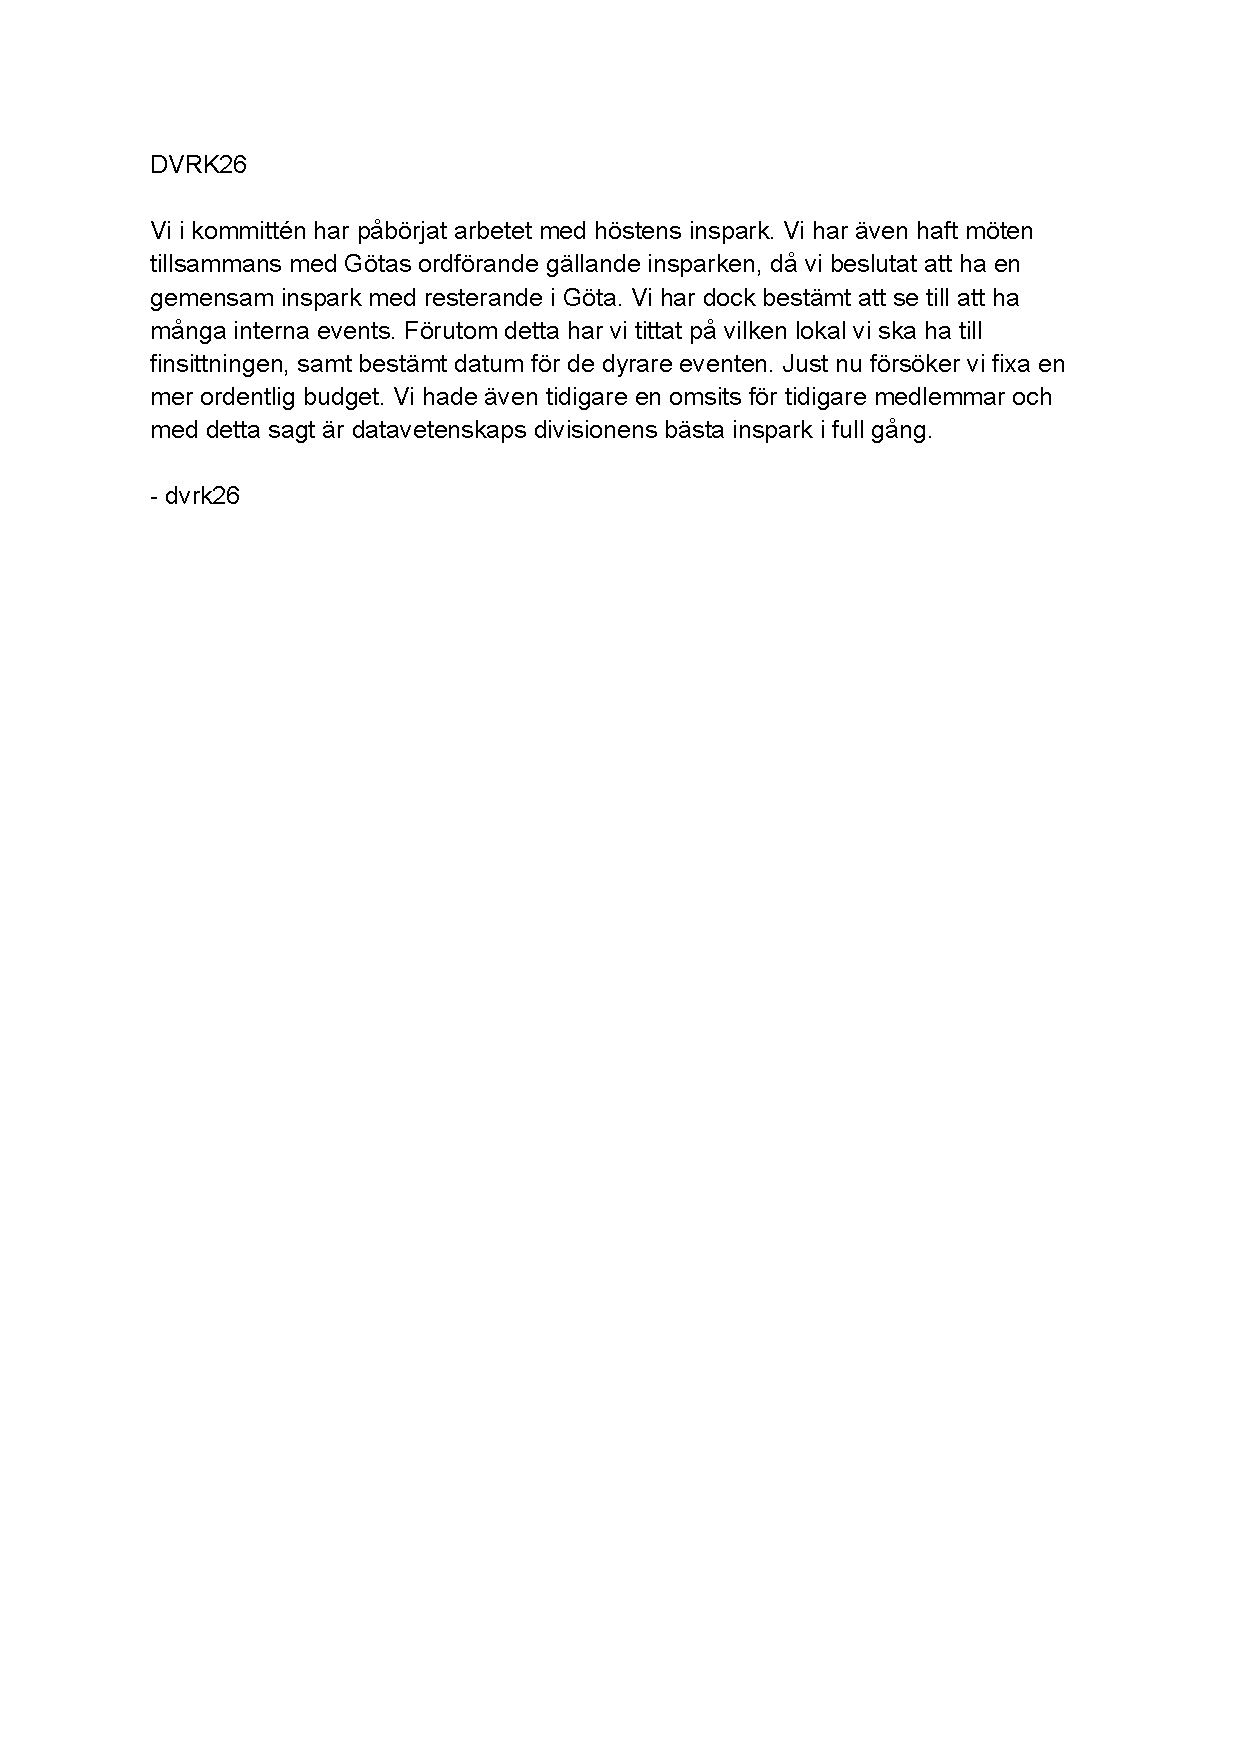
\includepdf[pages=-]{reports/dvrk26.pdf}

\subsubsection*{ConCats}
 ConCats har arrat några events nu med en filmkväll (som gick sådär) och en pluggstuga inför lp3 tentorna (var inte med) men som nämnt innan har vi äntligen ett steamdeck som förväntas att använda lite oftare än den gamla wii:et som nu ska samla damm i styrelserummet, utöver hade vi också behandlat sofforna (som skulle märkas) men gällande nya events tänker ConCats hålla ett kommade brädspelskväll (woooo) snart och kanske en testkörning spelkväll för steamdecket nån gång i framtiden

\subsubsection*{Femme++}
Inte gjort något men hoppas vi kan få igång något nu efter tentorna.

\subsubsection*{Mega6}
Har planer, bara fråga om när. 

\subsubsection*{DVOps}
Muntlig rapport.

\subsubsection*{Mega7}
Ingen rapport har inkommit.

\subsubsection*{Klubbsport DV}
Ingen rapport har inkommit.

\newpage

\section{Beslutspunkter}

Enligt Stadgan måste ändringar av Stadgan röstas igenom på två av Divisionsstämmans varandra följande möten.
Om en beslutspunkt innehåller ``första läsningen' innebär det att det är första gången beslutet tas upp för omröstning.
Om en beslutspunkt innehåller ``andra läsningen'' innebär det att beslutspunkten har röstats igenom förra stämmomötet, och beslutet behöver bekräftas för att gå igenom.
\\
Inga beslutspunkter på agendan. 


\subsection*{Motioner}
Inga motioner har tillkommit.

\newpage

\section{Inval}
Inval av personer till förtroendeposterna som väljs in av Divisionsstämman. Dessa väljs in för en ordinarie mandatperiod, vilket sträcker sig från 1 januari till 31 december.

\subsection*{DVArm}
\subsubsection*{Inkomna nomineringar inför mötet}
\textit{Styrelsen har ej fått in några nominering innan stämman.}
\subsubsection*{Fri nominering}
\subsubsection*{Förslag till beslut}
\begin{attsatser}
    \item punkten bordsläggs
\end{attsatser}
\subsubsection*{Beslut}
\begin{attsatser}
    \item attsats 1 bifalles
\end{attsatser}

\subsection*{Revisor}
\subsubsection*{Inkomna nomineringar inför mötet}
\textit{Styrelsen har ej fått in några nominering innan stämman.}
\subsubsection*{Fri nominering}
\subsubsection*{Förslag till beslut}
\begin{attsatser}
    \item punkten bordsläggs
\end{attsatser}
\subsubsection*{Beslut}
\begin{attsatser}
    \item attsats 1 bifalles
\end{attsatser}

\newpage
\section{Diskussionspunkter}
Stämman är inte bara en chans för oss i divisionen att rösta om saker, utan den ger oss även en chans att diskutera olika ämnen, som kanske nödvändigtvis inte behövs röstas om.

\\
\textit{Inga punkter har inkommit innan mötet, och styrelsen har ej kommit några punkter själva.}
\subsection*{DVD-logga i backen}
Det har varit en genomgående efterfrågan att måla DVDs logga på marken. På en tidigare stämma röstades det igenom att styrelsen förra styrelsen skulle kontakta Chalmers studentkår och undersöka om vi kunde måla DVDs logga i backen ovanför trappan där flera av Chalmers föreningar har sina. Det har också diskuterats att ha loggan på Rännvägen eller precis utanför Monaden. 

Styrelsen kontaktade studentkåren men fick aldrig något svar. 

Är detta något stämman vill att nya styrelsen undersöker igen och är det fortfarande i backen ovanför trappan där loggan önskas?

\\
Stämman önskar att detta skall undersökas i år igen. 

\subsection*{Jubileumsfirande}
Skulle ha varit ett förra året men det var ytterst få som anmälde sig. 
Punkten diskuterades på senaste kommittémöte där det föreslogs att, istället för en sittning, ha ett sorts mingel/grill i innergården. 
Vi skulle möjligtvis kunna använda pengarna vi fick som blev över från insparken till detta. 

Vi söker en arbetsgrupp som kan hjälpa till med planering et cetera. 

Preliminärt siktar på mitten eller slutet av maj.

\\ 
Stämman föreslog ett preliminärt datum av den 22:e maj.


\subsection*{Examensfirande}
De senaste åren har vi hållit ett grill-mingel för att hylla de som tagit examen och detta skulle vara en trevlig tradition att fortsätta.  
Detta är också något vi skulle kunna använda den överblivna insparks-budgeten till. 

Vi söker en arbetsgrupp som kan hjälpa till med planering et cetera. 

Preliminärt siktar på början av juni.

\\
Mer planering skall påbörjas senare. 


\newpage
\section{Avslutande av möte}

Mötet avslutades klockan 18:24

\stämmosignaturer

\end{document}
